\documentclass[11pt]{report}

% I want multiple citations to be condenced. ie. [1, 2, 3, 4] -> [1-4]
% I want back references in my bibliography.
\usepackage[backref = true, sorting = none, backend = bibtex, style=nature]{biblatex}
% Phrase the back reference nicely.
\DefineBibliographyStrings{english}{%
  backrefpage = {cited on page},
  backrefpages = {cited on pages},
}
% Links without boxes around them.
\usepackage[hidelinks]{hyperref}
% Color for... color.
\usepackage{color}
% Need this for figures
\usepackage{graphicx}
% This may include the bibliography in the table of contents
\usepackage[numbib]{tocbibind}
% Slightly neater way of doing units.
\usepackage{units}
% Glossary package for acronyms.
\usepackage[nonumberlist]{glossaries}%[nonumberlist,nohypertypes={glossary},acronym]
\setglossarysection{subsubsection} % No page break on \printglossary
\renewcommand{\glossarysection}[2][]{} % No glossary title.

\newacronym{cdi}
    {CDI}{coherent diffractive imaging}

\newacronym{odt}
    {ODT}{optical dipole trap}

\newacronym{otr}
    {OTR}{optical transition radiation}
    
\newacronym{bec}
    {BEC}{Bose-Einstein condensate}

\newacronym{fort}
    {FORT}{far-off-resonance trap}

\newacronym{ta}
    {TA}{tapered amplifier}

\newacronym{caes}
    {CAES}{cold-atom electron source}

\newacronym{cais}
    {CAIS}{cold-atom ion source}

\newacronym{caeis}
    {CAEIS}{cold-atom electron and ion source}

\newacronym{xfel}
    {XFEL}{X-ray free electron laser}

\newacronym{mot}
    {MOT}{magneto-optical trap}

\newacronym{ecdl}
    {ECDL}{external cavity diode laser}

\newacronym{aom}
    {AOM}{acousto-optic modulator}

\newacronym{eom}
    {EOM}{electro-optic modulator}

\newacronym{slm}
    {SLM}{spatial light modulator}

\newacronym{mopa}
    {MOPA}{master-oscillator power amplifier}

\newacronym{na}
    {NA}{numerical aperture}

\newacronym{ar}
    {AR}{anti-reflection}

\newacronym{ccd}
    {CCD}{charge-coupled device}

\newacronym{cro}
    {CRO}{cathode ray oscilloscope}

\newacronym{pbs}
    {PBS}{polarising beam splitter}

\newacronym{bs}
    {BS}{beam splitter}

\newacronym{npbs}
    {NPBS}{non-polarising beam splitter}

\newacronym{tec}
    {TEC}{thermo-electric cooler}

\newacronym{cw}
    {CW}{continuous wave}

\newacronym{mcp}
    {MCP}{microchannel plate}

\newacronym{fwhm}
    {FWHM}{full-width half maximum}

\newacronym{pdh}
    {PDH}{Pound-Drever-Hall}

\newacronym{ps}
    {PS}{polarisation spectroscopy}

\newacronym{psf}
    {PSF}{point spread function}

\newacronym{obe}
    {OBE}{optical Bloch equation}
    
\newacronym{davll}
    {DAVLL}{dichroic atomic vapour laser lock}

\newacronym{mts}
    {MTS}{modulation transfer spectroscopy}

\newacronym{snr}
    {SNR}{signal-to-noise ratio}

\newacronym{lsd}
    {LSP}{linear spectral density}
    
\newacronym{psd}
    {PSD}{power spectral density}
    
\newacronym{piezo}
    {PZT}{piezoelectric transducer}

\newacronym{rms}
    {RMS}{root mean square}
    
\newacronym{sa}
    {SA}{saturated absorption spectroscopy}

\newacronym{fib}
    {FIB}{focused ion beam}

\newacronym{rf}
    {RF}{radio frequency}
    
\newacronym{ued}
    {UED}{ultrafast electron diffraction}

\newacronym{tem}
    {TEM}{transmission electron miscroscopy}

\newacronym{fsr}
    {FSR}{free-spectral range}

\newacronym{rempe}
    {REMPE}{resonace-enhanced multiphoton excitation}

\newacronym{tcmpe}
    {TCMPE}{two-colour multiphoton excitation}
\makeglossaries

% Add the .bib file.
\bibliography{Library}

\begin{document}

% Title page
\title{Thesis}

\author{Joshua Torrance}

\pagenumbering{alph} % Title page becomes a so backrefs to 1 go to the right place.
\maketitle

\pagenumbering{roman}

% Front matter
\chapter*{Abstract}
\addcontentsline{toc}{chapter}{Abstract}

The understanding of atomic structures and processes is continually improving with the great technological development in imaging techniques.
Ultrafast electron and X-ray techniques are able to perform measurements at atomic lengths and timescales and both these techniques require the generation of high-brightness ultrashort-duration electron bunches.
Electron techniques directly use these short bright bunches and in \glspl{xfel} the electron bunches are used to generate short bright bunches of X-ray.

It is hoped that \glspl{caeis} will also be able to produce ultrashort high-brightness electron bunches that are brighter than current sources due to the unique method of generating electrons used by these sources.
\Glspl{caeis} generate electrons via near-threshold ionisation from an ultracold atomic gas and has been shown to create electrons bunches with temperature as low as \unit[10]{K}.
Conventional photocathode sources have temperatures of thousands of Kelvin and thus \glspl{caeis} have the potential to produce brighter electron bunches.
\Gls{caeis} are also capable of producing extremely cold ion bunches and show great promise as an ion source for ion milling and microscopy.

This thesis describes a number of developments involved with the \gls{caeis} project at the University of Melbourne, in particular pushing the boundaries of laser frequency stabilisation, and a new technique for measuring the brightness of charged particle bunches.
A number of smaller developments and investigations are presented along with the newest diffraction measurements.

Laser frequency stabilisation is an essential component of the \gls{caeis} and many other applications including metrology, spectroscopy and laser cooling.
The high-bandwidth of the laser stabilisation technique polarisation spectroscopy has not previously been fully utilised and by using high-bandwidth feedback laser linewidth can be narrowed to much less than \unit[1]{kHz}, two orders of magnitude better than previously reported.

Brightness is the most comprehensive figure of merit for charged particle beams and a new technique for measuring the brightness with time-resolution is presented.
The technique achieves time-resolved brightness measurements by streaking one-dimensional pepperpot measurements across the detector.
Time-resolved brightness measurements have the potential to reveal information related to the ionisation processes used in \glspl{caeis} and can show the efficacy of techniques used to counter the effects of space charge in the beams produced from a \gls{caeis}.

The performance of the \gls{caeis} apparatus operating in its normal pulsed mode is compared to continuous operation with a focus on the beam current and electron trajectory stability.
The beam quality was also improved by identifying an astigmatism in the beam and correcting it with a 3D printed quadrupole lens.
Virtually all the beam measurements presented here utilise the image processing techniques that allow for multi-shot averaging despite the inconvenient instabilities in the electron beam trajectories.

This iteration of a \glspl{caeis} was able to produce ultrashort-duration electron bunches and these have been used to demonstrate ultrafast electron diffraction from thin gold foils.
This is an important step along the path to being able to perform ultrafast single-shot \gls{cdi} and next iteration of the \gls{caeis} should have sufficient current to demonstrate \emph{single-shot} ultrafast diffraction and then move on to \gls{cdi}.
\chapter*{Acknowledgements}
\addcontentsline{toc}{chapter}{Acknowledgements}

Acknowledgements go here.

\chapter*{Contributions}
\addcontentsline{toc}{chapter}{Contributions}

This thesis presents work I was involved with as a member of the Atom Optics group in the School of Physics at the Unisversity of Melbourne.
All work in this thesis was conducted by me, unless mentioned below:
\begin{itemize}
\item The Cold-Atom Electron and Ion Source: The experimental apparatus was designed, contructed, and improved by other members of the group before my research with it began.
Some of the members of the group that have worked on the apparatus are
Andrew McCulloch, Dene Murphy, Corey Putkunz, Robert Scholten, David Sheludko, Sebastian Saliba, Ben Sparkes, Rory Speirs, Richard Taylor, and Daniel Thompson.
\item The high-bandwidth polarisation spectroscopy work described in Chapter~\ref{chapter:polspec} was conducted with much help and advice from Robert Scholten, Ben Sparkes as well as Lincoln Turner from Monash University. Alex Slavec from MOGLabs was also instrumental in this work as he engineered the high-bandwidth modifications for the MOGLabs lasers used.
\item The results described in Chapter~\ref{chapter:diffraction} built on work done by Rory Speirs, published in Reference~\cite{speirs_single-shot_2015}, and conducted with much advice from Rory.
\item The deflectors used to streak the electron beam in Chapter~\ref{chapter:emittance} were supplied a voltage with electronics designed and built by Rory Speirs and the deflector plates were designed by Andrew McCulloch.
\end{itemize}

\tableofcontents

 \chapter{Introduction}
 
\pagenumbering{arabic}
\setcounter{page}{1}

Molecular imaging has provided science with great advances during it's history, such as X-ray crystallography determining the helical structure of DNA in 1953~\cite{watson_molecular_1953} and structure of myoglobin and haemoglobin in 1962~\cite{kendrew_x-ray_1957}.
The \gls{caeis} at the University of Melbourne is an ongoing project that aims to develop a source capable of achieving the `holy grail' of scientific imaging, the `molecular movie'~\cite{dwyer_femtosecond_2006,sciaini_femtosecond_2011}.
A \gls{caeis} also has potential applications with \gls{fib} techniques~\cite{mcclelland_bright_2016}, and as particle source for accelerators such as synchrotrons and \glspl{xfel} for \gls{cdi} of non-crystalline targets~\cite{van_oudheusden_electron_2007, zhu_future_2015, mcculloch_cold_2016}.



{\color{red}
Some kind of introduction for everything will go here.

Motivate CAES. Imaging of things is important. Membrane proteins, cystallisation. What else can we image with it? What else can we study with it? Ion source.

Briefly motivate part 1 and part 2.}

\section{Making the `Molecular Movie'}

Being able to observe molecular dynamics at an atomic spatial and temporal scale could provide great insight into some of the basic processes of biology and chemistry.
The fabled `molecular movie' refers to capturing the atomic motions of molecular systems as they undergo some transition such as a chemical reaction, protein folding or melting.
Molecular movies could provide greater understanding of important biological reactions such as photosynthesis or oxygen transport by haemoglobin.

One of the stepping stones towards molecular movies is single-shot imaging of non-crystalline molecules which would allow structural determination of membrane proteins, an essential step in rational drug design~\cite{hardy_atomic_1987, barrett_discovering_1999, pinto_influenza_1992}.
One of the main techniques in stuctural determination of crystalline targets is electron diffraction which, along with X-ray and neutron methods~\cite{cullity_elements_2001,bacon_x-ray_2013}, has be utilised in structural determination of many materials with atomic resolution.
Continuing research into real-space and diffraction imaging techniques is aiding in the understanding of a growing range of samples as well as providing new types of information on the sample under investigation.

Ultrafast imaging techniques are a relatively recent development and they provide the opportunity to study electronic and atomic dynamics.
Ultrafast techniques also provide an avenue for the imaging of structures that, to date, cannot be imaged by cyrstallographic techniques as some of these techniques should be applicable to uncrystallised samples with imaging being faster than damage processes~\cite{gaffney_imaging_2007,barty_ultrafast_2008,miao_beyond_2015}.
In the past the greatest success with structural determination has been acheived with crystallography which is limited by to samples that can be crystallised.
There are a large number of biological proteins of interest, particularly membrane proteins, that cannot be crystallised and developements in ultrafast imaging techniques is providing a route towards structural determination without crystallisation~\cite{dauter_current_2006,levitt_nature_2009}, cryogenic electron microscopy is also making headway in this area~\cite{henderson_model_1990,zhou_towards_2008}.
Both X-ray and electron imaging techniques are limited by the capabilities of their sources which are undergoing continual developement, in the realms of fundamental physics and engineering.
The techniques using X-rays and electrons each have different advantages and disadvantages with regards to dynamic imaging and structural determination and they often give complementary information.

Some recent results from X-ray sources are well on the way to producing molecular movies~\cite{pande_femtosecond_2016,nango_three-dimensional_2016}.

\subsection{Imaging Targets}

Membrane proteins.
Chemical reactions.


\subsection{Requirements}

Ultra-fast, single-shot, orientation, flux, coherence.

\subsection{X-rays}

XFELs

\subsection{Electrons}

\subsection{Pump-Probe}

\section{Cold-atom electron sources}

\subsection{Developments}

Arbitrary shaping, charged partical dynamics, diffraction.
\subsection{Ion Source}

\section{Thesis Outline}

\subsection{Part I}

\subsection{Part II}

% The following two lines need to be in the first chapter to get Arabic page numbers.
%\pagenumbering{arabic}
%\setcounter{page}{1}
\part[Polarisation Spectroscopy]{Polarisation Spectroscopy\\
\vspace{1cm}
\LARGE Pushing the Limits of Polarisation Spectroscopy as a Laser Frequency Reference}
\chapter{Introduction}

Laser frequency stabilisation is an essential tool for atomic physics experiments, without it experiments involving \glspl{bec}, atomic clocks and many more would not be possible~\cite{anderson_observation_1995,ye_quantum_2008}.
There are a plethora of techniques available for laser frequency stabilisation each with numerous advantages and disadvantages.

\Gls{ps} is one such technique that will be discussed in detail~\cite{demtroder_laser_2003}.
\Gls{ps} was first described by Wieman and H\"anch in 1976 as, ``...a sensitive new method of Doppler-free spectroscopy, monitoring the nonlinear interaction of two monochromatic laser beams in an absorbing gas via changes in light polarisation."~\cite{wieman_doppler-free_1976}
This chapter provides an overview of laser frequency stabilisation, a detailed discussion of the physics of \gls{ps} followed by details on the implementation and measurement of high bandwidth frequency stabilisation using \gls{ps}.

\section{Laser Frequency Stabilisation}

Laser frequency stabilisation describes a number of techniques that are used to reduce the temporal frequency spread of a laser's frequency.
This can range from weak frequency stabilisation keeping the centre frequency of a laser at a particular point to convoluted frequency narrowing techniques that attempt to reduce laser linewidth to sub-hertz levels.
Typically these techniques use some reference to measure frequency deviation from a given frequency and provide negative feedback to the laser, using a servo system, to keep it at the target frequency.

The efficacy of stabilisation techniques can be described by width of the frequency distribution of the laser, called the linewidth.
Width is usually refers to either the \gls{fwhm} or \gls{rms} width about the central frequency.
Linewidth can describe short or long timescale measurements.
Short measurements, usually less than a second measurement, are used to describe the linewidth of laser whereas long timescale measurement, hours or days in duration, are used to describe the drift of the laser central frequency over time.

There are a number of traits that are desirable in a laser frequency stabilization scheme including the ability to stabilize to an absolute atomic reference, absence of frequency or amplitude modulation, high bandwidth to achieve low spectral linewidth, large capture range, low complexity and low cost.

There are a large number of available techniques and variations on techniques for stabilization each with different advantages and drawbacks.
These techniques include
\begin{itemize}
\item \gls{sa}~\cite{haroche_theory_1972, maguire_theoretical_2006, cuneo_optically_1994, preston_doppler-free_1996, saliba_linewidths_2009},
\item \gls{davll}~\cite{corwin_frequency-stabilized_1998, millett-sikking_davll_2007},
\item \gls{mts}~\cite{shirley_modulation_1982, mccarron_modulation_2008, xiang-hui_ultra-stable_2009},
\item Sagnac interferometry~\cite{robins_Interferometric_2002, jundt_non-linear_2003},
\item \acrfull{ps}~\cite{wieman_doppler-free_1976, lancaster_polarisation_1999, yoshikawa_frequency_2003, harris_polarization_2006, pearman_polarization_2002, tiwari_laser_2006, do_polarization_2008, torii_laser-phase_2012}
\item \gls{pdh}~\cite{drever_laser_1983} and
\item H\"ansch Couillaud stabilisation~\cite{hansch_laser_1980}.
\end{itemize}
Some of these techniques will be discussed later on in this chapter.

\section{Feedback Methods}

Stabilisation techniques require some kind of feedback to the laser in order to keep it at the desired frequency.
There are a few common ways of providing feedback to lasers, the focus here will be on diode lasers, particularly \glspl{ecdl}.

\subsection{Current Feedback}

Diode lasers require an electric current in order to function and this current can be used to control the output frequency of the laser.
The front and rear facets of laser diodes are reflecting forming an optical cavity.
The optical cavity support standing waves of particular wavelengths which serve to enhance the stimulated emission essential to lasing.
The electrical current passing through a laser diode will cause an increase in temperature of the diode which in turn increases the size of the cavity and the supported standing wave wavelength.
Increasing the temperature also affects the band gaps in the crystal such that an increase in temperature causes an increase in wavelength.
Thus altering the current supply to the laser can be use to control the central output frequency of the laser.

{\color{red} Verify these and provide citations.}

To talk about:
\begin{itemize}
\item Typical feedback bandwidths.
\item Grating feedback.
\item Fast feedback - complications (isolation from ground, phase lag...).
\end{itemize}


\section{Noise}
Thermal noise can affect the alignment of optics, the efficiency and polarisation of light transmitted through fibres, atomic vapour cell opacity and the intensity and frequency of light emitted from laser diodes, not to mention mode hops.

Noise in the electronic environment can also cause frequency instability. Noise on the power supply to the laser diode affects the intensity and frequency of the light emitted.

In certain applications {\color{red}(such as?? imaging?)} intensity noise can be as much as a drawback as frequency noise and with some frequency discrimination methods intensity noise is interpreted as frequency noise which the servo would then attempt to correct for thus inducing frequency noise.

Feedback to laser systems typically takes the form of modulation of either the current supply to the diode or the voltage to a piezo that controls the angle of the grating in an \gls{ecdl}.
Temperature feedback has also been used to maintain frequency stability {\color{red}[find that paper again]}.
The bandwidth of current feedback tends to range from \unit[0]{Hz} to MHz~\cite{ludlow_compact_2007}{\color{red}[cite my paper here?]}.
Piezo response is significantly slower ranging from \unit[0]{Hz} to \unit[100]{kHz}.

{\color{red}Frequency ranges of noise.}
{\color{red}More detail? More References on noise in general.}

Bleh.
\Glspl{ecdl} subjected to mechanical vibrations will experience frequency noise as the alignment of the light coupled back into the diode off the grating varies.
Vibrations can also affect the alignment, and thus transmitted power, of laser through optical fibres, optical isolators and through apertures.

\section{Stabilisation Techniques}
\subsection{Saturated Absorption Spectroscopy}
\Gls{sa} is a simple and common technique for laser frequency stabilisation~\cite{demtroder_laser_2003}.
 
\begin{figure}
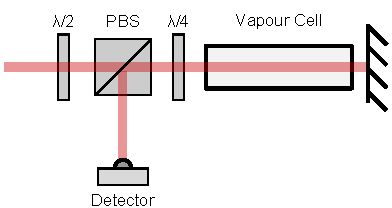
\includegraphics[width=\linewidth]{part1/Figs/SatAbs.pdf}
\caption{Saturated absorption spectroscopy.}
\label{figure:satabs}
\end{figure}

\subsection{Polarisation Spectroscopy}

Summary of PS.

Pol Spec developments

It has been shown previously that \gls*{ps} can be used to reduce the linewidth of a distributed feedback diode from \unit[2]{MHz} to \unit[20]{kHz}~\cite{torii_laser-phase_2012} and of \glspl*{ecdl} to \unit[65]{kHz}
~\cite{yoshikawa_frequency_2003}.

Balanced polarimeter.\cite{pearman_polarization_2002,yoshikawa_frequency_2003}

Bi-polarisation spectroscopy.\cite{tiwari_laser_2006}


\subsection{Pound Drever Hall}

The \gls{pdh} technique is the standard for laser frequency linewidth reduction.\cite{drever_laser_1983}
\gls{pdh} uses an optical cavity as a frequency reference and an \gls{eom} to modulate the the light incident to the cavity.

More detail. Some maths. What linewidth can it achieve?\cite{ludlow_compact_2007}

\begin{figure}
\centering
\includegraphics[width=\linewidth]{part1/Figs/pdh.jpg}
\caption{A beautiful \gls{pdh} schematic.}
\end{figure}
\subsubsection{Dichroic Atomic Vapour Laser Lock}
\Gls{davll} works by....

It can achieve linewidths of....

\subsection{Modulation Transfer Spectroscopy}
\Gls{mts}...

It can achieve linewidths of...\cite{negnevitsky_wideband_2013}

\subsection{Other Techniques}

Any others?



\chapter{Polarisation Spectroscopy}\label{section:pol_spec_theory}
\section{Basic Theory}

In \gls{ps} a circularly polarised pump beam from a monochromatic laser, with frequency close to an atomic resonance, induces frequency-dependent circular birefringence in a magnetically-shielded atomic gas sample.
A linearly polarised beam from the same source is used to measure the birefringence, monitored with a balanced polarimeter consisting of a half-wave phase retarder, \gls{pbs} and two detectors.
This is shown in Figure \ref{figure:pol_spec_schematic}.

\begin{figure}
\centering
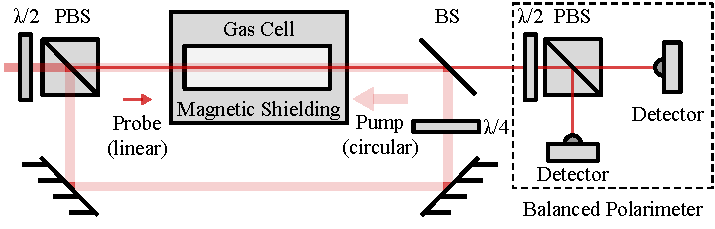
\includegraphics[width=\linewidth]{part1/Figs/PolSpecSchematic.pdf}
\caption{A schematic of \gls{ps} with a balanced polarimeter.
The power balance between the probe and the pump beam is controlled with the left-most $\lambda/2$ phase retarder and \gls{pbs}.
The $\lambda/4$ retarder is adjusted to produce a circularly polarised pump beam.
The non-polarising beamsplitter (BS) is used to counter-propagate the pump beam through the atomic sample without altering the polarisation of the circular pump or linear probe.
The final $\lambda/2$ retarder, \gls{pbs} and the detectors form the balanced polarimeter that monitors the polarisation rotation of the probe.}
\label{figure:pol_spec_schematic}
\end{figure}

The circularly polarised pump beam induces circular birefringence in the atomic sample by partially optically pumping the sample into one of the extreme hyperfine sublevels, $m_F=\pm F$, where $m_F$ labels the hyperfine sublevel and $F$ labels {\color{red}some quantum thingy.}
This partial optical pumping, referred to here as the anisotropy of the medium, results in unequal absorption coefficients for each circular polarisation.
The linearly polarised probe beam can be decomposed into two equal and oppositely circularly polarised components which undergo different absorption due to the anisotropy, such that when recombined after passing through the atomic sample the probe beam becomes elliptically polarised with an angle different to that of the original linear polarisation.
This process is depicted in Figure \ref{figure:pol_spec_explanation}.

\begin{figure}
\centering
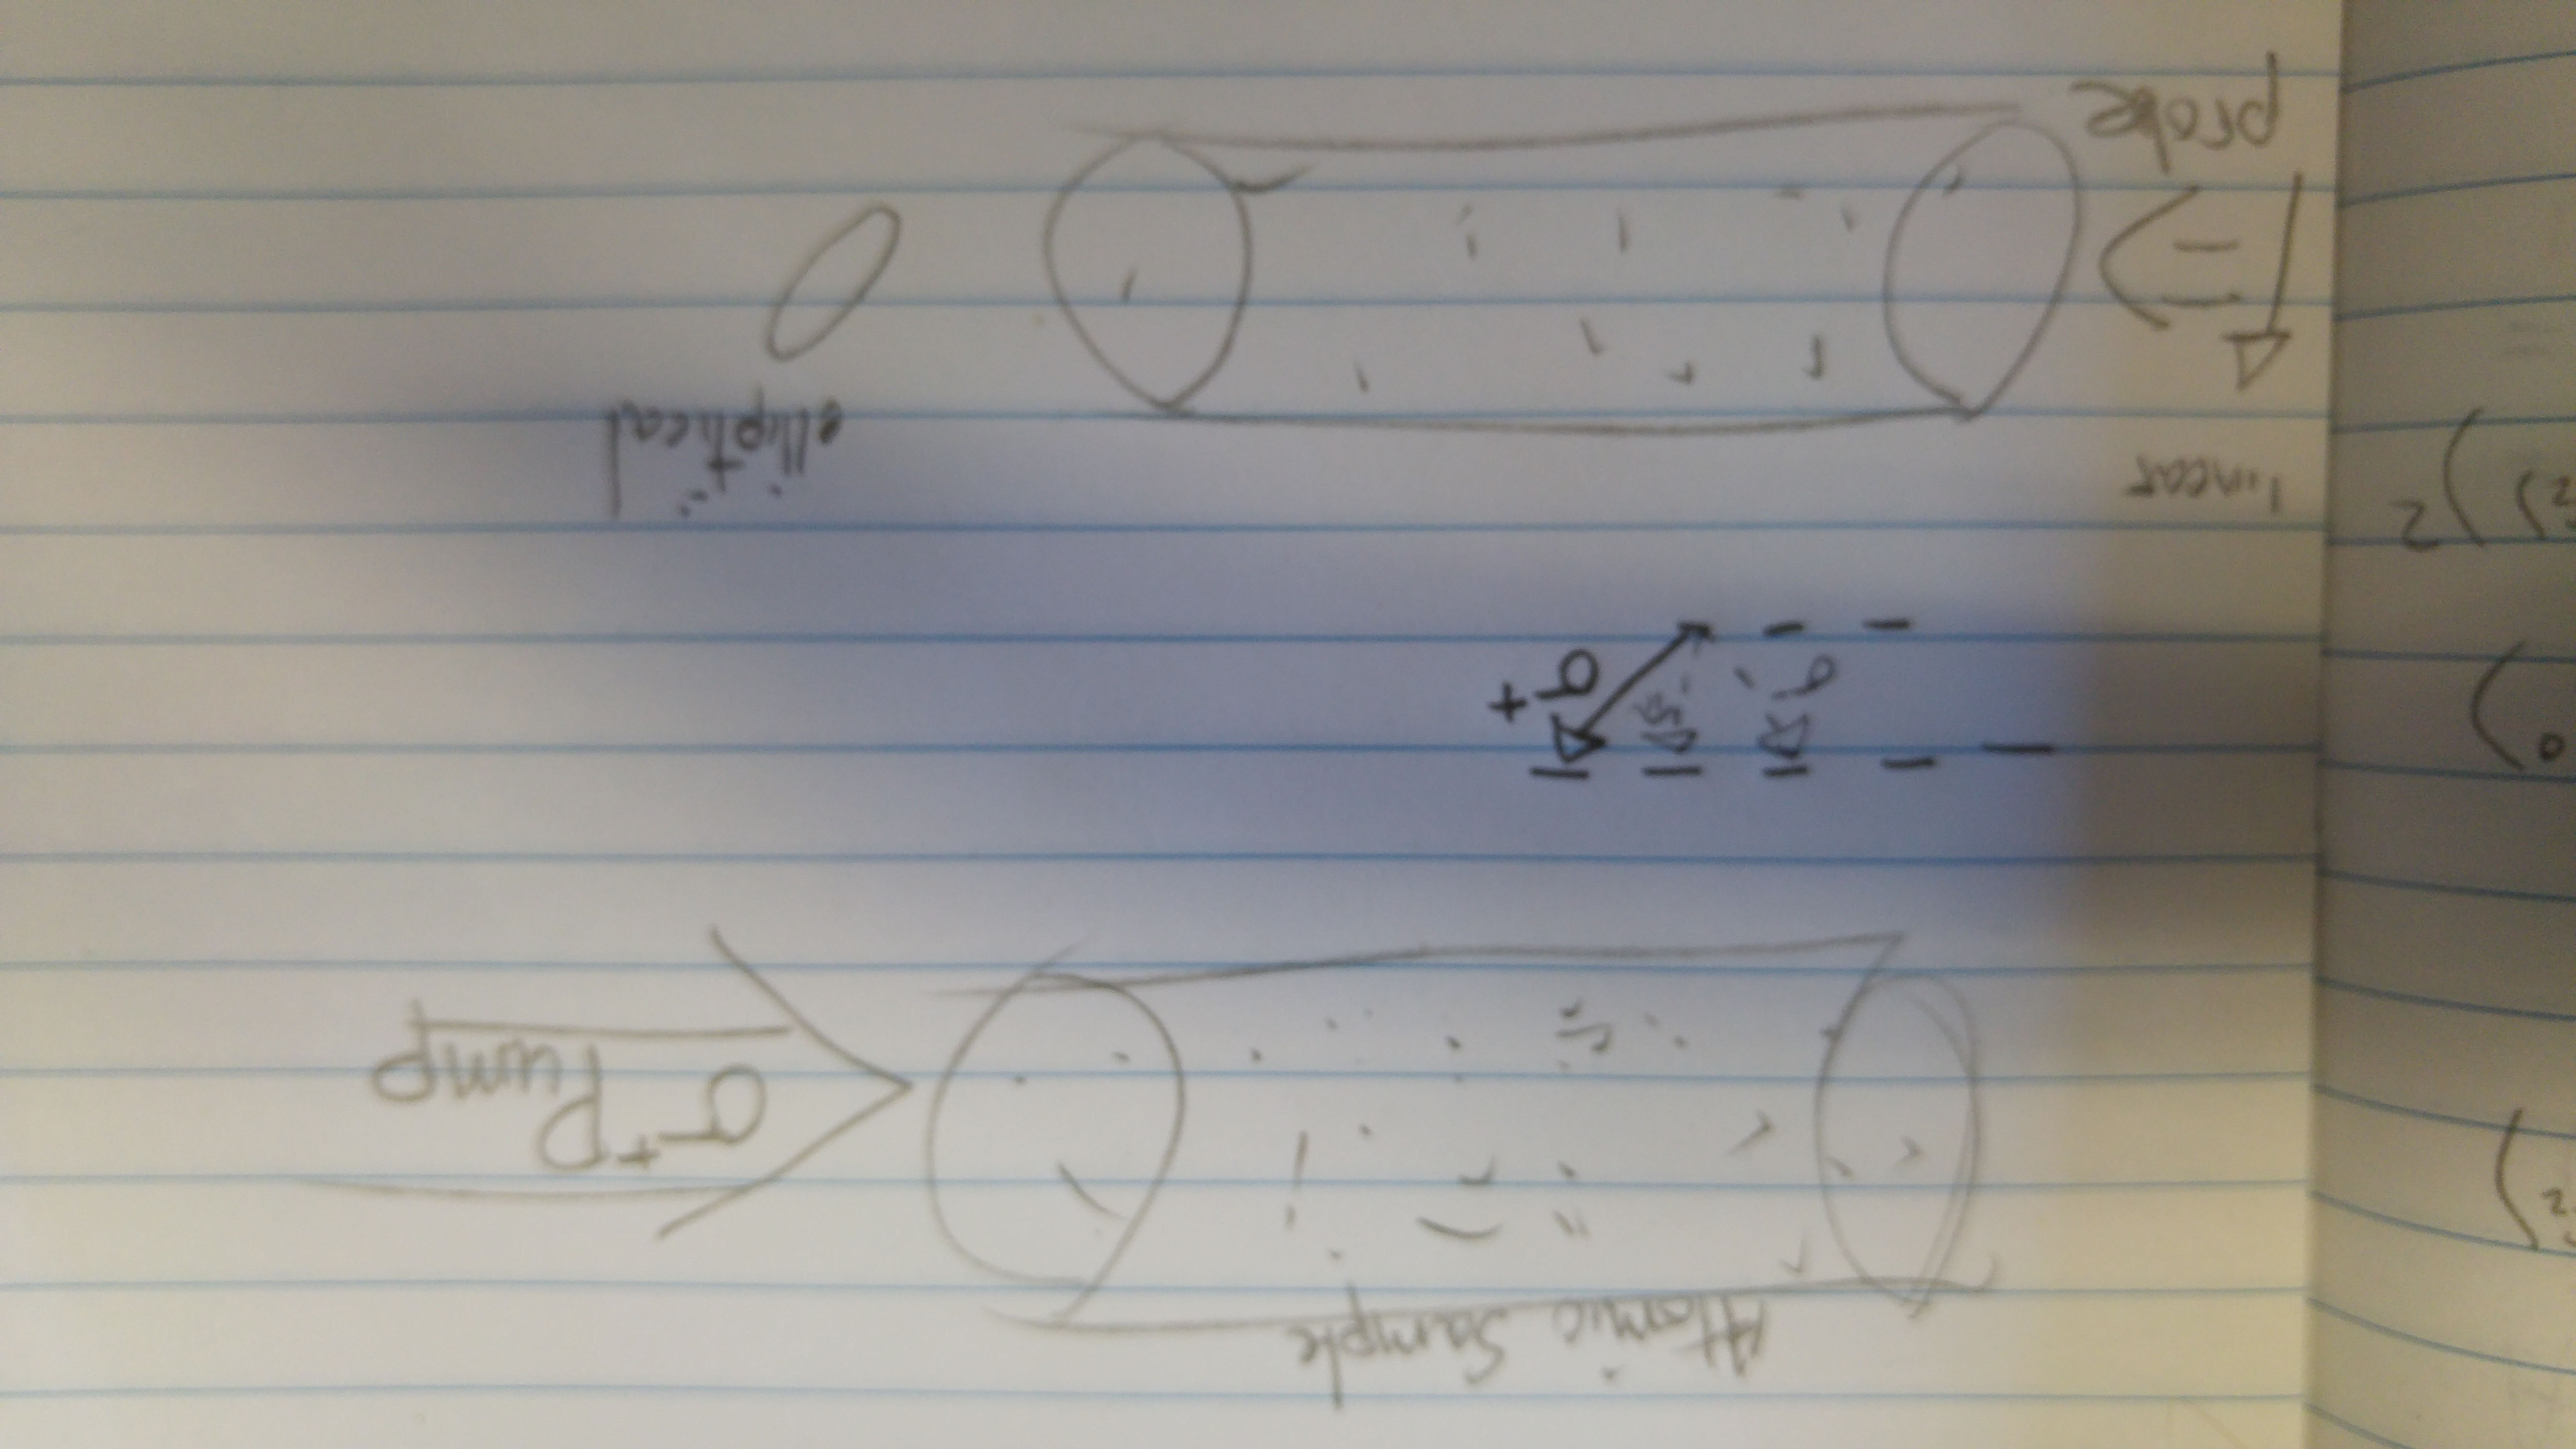
\includegraphics[width=\linewidth,angle=180]{part1/Figs/pol_spec_explanation_placeholder.jpg}
\caption{A conceptual figure for explaining the basics of pol spec.}
\label{figure:pol_spec_explanation}
\end{figure}

Consider the electric field of the probe beam before it enters the atomic sample at an angle $\phi$ to the $x$ axis:
\begin{equation}
\vec{E}=E_0\big(\cos{\phi}\,\hat{x}+\sin{\phi}\,\hat{y}\big)
\end{equation}
which can be expressed in terms of the circularly polarised basis vectors:
\begin{equation}
\vec{E} = \frac{E_0}{2}e^{-i\phi}(\hat{x}+i\hat{y}) + \frac{E_0}{2}e^{+i\phi}(\hat{x}-i\hat{y})
\end{equation}

After propagating through an atomic sample of length $L$ with refractive indices for the circular polarisation components of $n_\pm$, $\vec{E}$ and absorption coefficients of $\alpha_\pm$ the electric field becomes
\begin{align}
\vec{E} = &\frac{E_0}{2}e^{-i\phi}(\hat{x}+i\hat{y})\,\exp\left[\frac{i\omega n_+ L}{c} - \frac{\alpha_+ L}{2}\right] +\notag\\
&\frac{E_0}{2}e^{+i\phi}(\hat{x}-i\hat{y})\,\exp\left[\frac{i\omega n_- L}{c} - \frac{\alpha_- L}{2}\right]\label{equation:elliptically_polarised}
\end{align}

Equation \ref{equation:elliptically_polarised} represents elliptically polarised light with the major axis at an angle of $\theta$ to the $x$-axis, where
\begin{equation}
\theta = \phi + \frac{\pi L (n_+ - n_-)}{\lambda}
\end{equation}
thus the angle by which the probe has rotated is
\begin{equation}
\Phi = \frac{\pi L \Delta n}{\lambda},
\end{equation}
where $\Delta n = n_+ - n_-$.

The electric field after the sample can be approximated to {\color{red}(probably don't need to make this approximation going from 1.3 to 1.7)}
\begin{equation}
\vec{E} = E_0\big(\cos\left[\phi+\Phi\right]\,\hat{x}+\sin\left[\phi+\Phi\right]\,\hat{y}\big).
\end{equation}

The output of the balanced polarimeter is the difference between the intensity {\color{red}(P?)} of light incident on each detector:
\begin{align}
I_{out} = I_x - I_y &= \frac{1}{2}\epsilon_0 c \left(|E_x|^2 - |E_y|^2\right)\notag\\
&= \frac{1}{2}\epsilon_0 c \left(\cos^2\left[\phi+\Phi\right] - \sin^2\left[\phi+\Phi\right]\right)\notag\\
&= \frac{1}{2}\epsilon_0 c \cos\left[2\phi+2\Phi\right]\notag\\
&= I_0 \cos\left[2\phi+2\Phi\right]
\end{align}

The largest spectrum is provided when $\phi=\pi/4$ and since $\Phi$ is small $I_out$ can be approximated to
\begin{equation}
I_{out} = I_0 2\Phi = I_0 \frac{2\pi L \Delta n}{\lambda}
\end{equation}

\subsection{Theory from paper - to be merged}
A schematic diagram for polarization spectroscopy is shown in Fig.~\ref{polspec_schematic}.
A circularly polarized pump beam from a monochromatic laser induces frequency-dependent circular birefringence in a magnetically-shielded atomic gas sample.
A linearly polarized beam from the same source is used to measure the birefringence, monitored with a balanced polarimeter consisting of a half-wave phase retarder, \glsfirst*{pbs} and two detectors.
The difference, or error, signal from the two detectors is of the form \cite{pearman_polarization_2002}
\begin{align}
P_{PS} = P_x-P_y = -P_0 \cos(2\phi+2\Phi)\label{P_PS}
\end{align}
where $P_{x,y}$ are the power of the horizontal and vertical linearly polarized components of the probe after the sample, $P_0$ is the power of the probe in the absence of a pump beam, $\phi$ is the angle of polarization of the probe in the absence of a pump beam and $\Phi$ is the additional polarization rotation of the probe due to the birefringence induced by the pump.
The largest \gls*{ps} spectrum is produced when $\phi=\pi/4$ and since $\Phi$ is small Eq.~(\ref{P_PS})  becomes
\begin{align}
P_{PS} = 2P_0 \Phi.
\end{align}
The polarization rotation is given by
\begin{align}
\Phi = \frac{\pi L \Delta n}{\lambda},
\end{align}
where $L$ is the length of the atomic sample, $\lambda$ is the wavelength of the light, $\Delta n = n_+ - n_-$ and $n_\pm$ are the refractive indices affecting the circularly polarized components of the probe beam $\sigma^\pm$.
\begin{figure}[htbp]
\centering
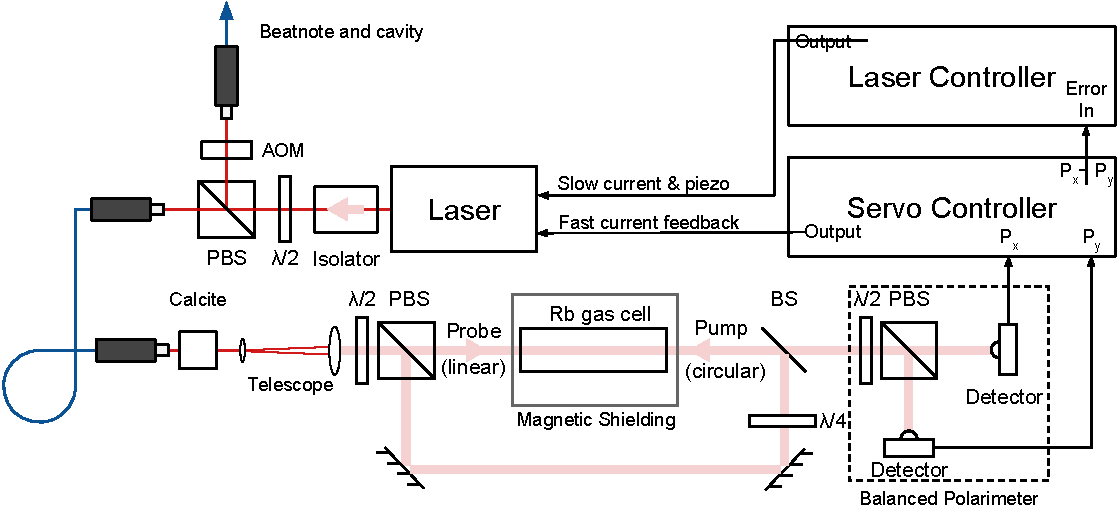
\includegraphics[width=\linewidth]{part1/Figs/fig1.pdf}
\caption{Schematic of a polarization spectroscopy (PS) apparatus.
The beam from the ECDL laser passes through an isolator before being split into two beams by a polarizing beam cube (PBS) and coupled into optical fibers.
One fibre leads to the PS setup and the other to other measurement or experimental apparatus.
The PS setup  consists of a polarization stabilizing calcite prism followed by a beam expanding telescope.
The expanded beam is then divided by a PBS into a linearly polarized probe and circularly polarized pump which counter-propagate, via a non-polarizing 50:50 beamsplitter (BS), through the magnetically shielded atomic gas sample.
The polarization rotation of the probe beam is then measured by a balanced polarimeter which consists of a $\lambda/2$ waveplate, PBS and two detectors.}
\label{polspec_schematic}
\end{figure}

The spectral profile of the difference in absorption coefficients for the circularly polarized components for the atomic medium in the vicinity of a resonance is a Lorentzian with width $\Gamma$, the inverse lifetime of the excited state of the resonant transition~\cite{demtroder_laser_2003}:
\begin{align}
\Delta \alpha = \frac{\Delta\alpha_0}{1+4\left(\frac{\delta}{\Gamma}\right)^2}.
\end{align}
Here $\delta=\omega_L-\omega_A$ is the detuning of the laser from the resonance, $\omega_L$ is the angular frequency of the laser and $\omega_A$ the angular frequency of the atomic resonance.
$\Delta\alpha_0$ is the difference in absorption coefficients for the $\sigma^\pm$ circular polarization components at zero detuning.

The refractive index and absorption of the medium are related through the Kramers-Kronig dispersion relation \cite{demtroder_laser_2003},
\begin{align}
\Delta n = \Delta\alpha_0 \frac{2c}{\omega_A \Gamma}\frac{\delta}{1+4\left(\frac{\delta}{\Gamma}\right)^2}.\label{result}
\end{align}
$\Delta\alpha_0$ is the sum over all $m_F$ ground states of the difference between absorption coefficients for each circular polarization, with $\delta=0$, weighted by the ground ($F, m_F$) and excited state ($F', m_{F\pm1}$) population differences,
\begin{align}
\Delta\alpha_0 = \sum_{m_F=-F}^{+F} \big[\alpha_{(F,m_F\rightarrow F',m_{F+1})}(P_{F,m_F}-P'_{F',m_{F+1}})\nonumber\\
-\alpha_{(F,m_F\rightarrow F',m_{F-1})}(P_{F,m_F}-P'_{F',m_{F-1}})\big].
\end{align}
The absorption coefficient for a given transition is $\alpha_{(F, m_F\rightarrow F',m_{F\pm1})}=N \sigma(\omega_L)$ where $N$ is the total number of interacting atoms, $\sigma(\omega_L)$ is the absorption cross section for the transition and $P_{F,m_F}$ refer to the populations of the various atomic states.

\subsection{Magnetic shielding}

\section{Fast Theory}

\subsection{from paper}
The atomic substate populations can be calculated using \glspl*{obe}~\cite{hughes_polarization_2009} but the standard steady-state solutions provide little insight into the behavior of the error signal when $\delta$ is changing faster than the evolution of the populations.
That evolution is limited to the spontaneous decay rate $\Gamma$, and hence for times $t\ll \tau=1/\Gamma$, the populations can be considered constant.
The \gls*{ps} signal is proportional to the refractive index difference given by Eq.~(\ref{result}), which describes a steep, background-free antisymmetric dispersive function, with bandwidth $1/t$ that can be much greater than $\Gamma$ (Fig.~\ref{sa_ps_spectra}).
Absorption-based frequency stabilization techniques such as \gls*{sa} rely on frequency-dependent changes to the atomic populations, rather than on the refractive index, resulting in dispersive signals over a much smaller capture range, with bandwidth limited to $\Gamma$.
SA is further limited if there are closely spaced hyperfine resonances or cross-over peaks.
Laser frequency noise can extend to frequencies much greater than $\Gamma$, where polarization spectroscopy still provides strong feedback and therefore can achieve much narrower laser linewidth.

\section{OBEs (timescale of state evolution, step in simulating)}

\section{Developments}

\subsection{Balanced Polarimeter}
When Wieman and H\"anch~\cite{wieman_doppler-free_1976} originally described \gls{ps} polarisation rotation was monitored with a nearly crossed polariser as shown in Figure \ref{figure:wieman_doppler-free_schematic}.
The polariser is crossed such that only a small proportion of the probe beam passes through them in the absence of the pump.
With the pump inducing anisotropy the rotation of the probe can be detected after the polarisers.

\begin{figure}
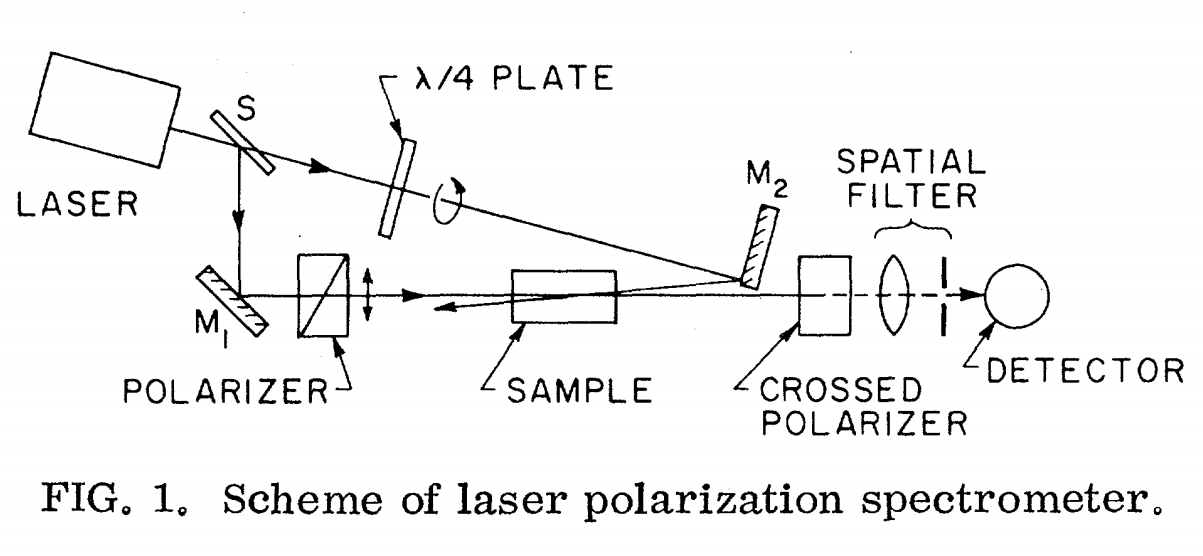
\includegraphics[width=\linewidth]{part1/Figs/wieman_doppler-free_schematic.png}
\caption{Figure stolen from Wieman and H\"anch paper.
Should probably redraw so I'm not plagiarizing.
Or ask how to cite it probably or some such.}
\label{figure:wieman_doppler-free_schematic}
\end{figure}

Pearson et al. proposed the alternative method of using a balanced polarimeter which provides a background-free signal with peak-to-peak height more than an order of magnitude greater than with the crossed polariser method~\cite{pearman_polarization_2002}.

\subsection{Beam splitter to co-propagate}

All papers thus far have ``snuck'' the pump beam through the vapour cell.

Figure with ``snucked'' and beam splitter configuration.

The angle of ``snucking'' has implications that there is math for...

Using a NBPS instead means you have an angle of 0.
The beam splitter has no effect on the polarisation as far as I can tell.

Pumped spectroscopy techniques such as \gls{ps} and \gls{sa}... spectral broadening due to angle stuff.

\subsection{High bandwidth feedback}


\subsection{Lincoln's magic detectors?}

\section{Experimental Setup (with details - fibres, calcite, etc.)}
\subsection{from paper - merge}
Two commercial Littrow configuration \glspl*{ecdl} were individually locked using \gls*{ps}.
The laser beam for each was split by a \gls*{pbs} and propagated through polarization-maintaining fibers to the \gls*{ps} locking system and linewidth measurements.
The locking beams were polarized with Glan-Thompson prisms (Fig.~\ref{polspec_schematic}) to eliminate residual polarization drift in the fibers.
Beam expanding telescopes were used to expand the beam to fill the apertures of the magnetic shielding, approximately \unit[1]{cm} diameter, allowing them to interact with more atoms to increase $|\Delta\alpha_0|$ and improve the \gls*{snr}.

The \gls*{pbs} balanced polarimeter error signal was generated with biased photodiodes (\unit[150]{MHz} bandwidth) and servo controllers (\unit[14]{MHz} bandwidth).
The servo controller integration zero-gain frequency was typically between \unit[100]{kHz} and \unit[1]{MHz}.
The diode modulation could be DC-coupled, with bandwidths of \unit[40]M{Hz} and \unit[10]{MHz}, or AC-coupled, \unit[100]{kHz}\,\textendash\,\unit[40]{MHz} and \unit[10]{kHz}\,\textendash\,\unit[10]{MHz}, depending on the laser.
The laser electronics provided control of the \glspl*{ecdl} piezoelectric transducer and diode injection current, with bandwidths of \unit[1]{kHz} and \unit[50]{kHz} respectively.



\chapter{Measurement Techniques}
We have characterized the performance of \gls*{ps} frequency stabilisation using a number of methods which are detailed here. Spectral linewidth is the principle metric by which stabilisation techniques are compared...

{\color{red}More detail in this intro.}

\section{Heterodyne Methods}

Heterodyning is a technique, invented by Canadian Reginald Feessenden in 1901, which mixes two frequencies to produce a new frequency. {\color{red} [get proper citation, this is from Wiki]} In optics the technique can be used to examine the spectral properties of two lasers.~{\color{red}[Citation?]}

\subsection{Basic Theory}
In the electrical signals context heterodyning involves the `mixing' or multiplying of two signals (e.g. two sine waves) to produce two different signals with frequencies equal to the difference and sum of the original frequencies:
\begin{equation}
\sin(\theta_1)\sin(\theta_2) = \frac{1}{2} \cos(\theta_1-\theta_2) - \frac{1}{2} \cos(\theta_1+\theta_2).
\end{equation}

In the optical context this is achieved due to the interference term accrued when squaring the electric field in order to calculate the intensity detected by the photodetector. The intensity of an electric field is given by:
\begin{equation}
I(t) = \frac{c\epsilon_0}{2}|E|^2.
\end{equation}

For two copropagating lasers with electric fields $E_{1, 2}$ and angular frequencies $\omega_{1, 2}$ we can write
\begin{equation}
E_{i}(t) = \sin(2\pi \omega_{i}).
\end{equation}
The electric field at the detector, $E_T$, is given by the sum of $E_{1}$ and $E_{2}$, and thus the intensity is given by,
\begin{align}
I(t) &= |E_1(t) + E_2(t)|^2\nonumber\\
&= E_1(t)^2 + E_1(t)E_2(t) + E_2(t)^2.
\end{align}
The interference, $E_1(t)E_2(t)$, term allows heterodyning of optical signals.

\subsection{Optical Heterodyne Methods}

There are a number of linewidth measurement techniques that utilise heterodyning. The major ones are:
\begin{itemize}
\item Heterodyne beatnote with two identical lasers.
\item Heterodyne beatnote between laser of interest and a relatively narrow reference laser.
\item Self-heterodyne beatnote of a laser with itself.
\end{itemize}

\subsection{Linewidth Discrepancies}
There is an interesting discrepancy between intuition and what the literature uses to describe `linewidth'.
Intuitively, when discussing the spectral properties of light, one would expect references to refer to the properties of the electric field since that is the entity that is interacting with atoms and other frequency references.
However, the literature seems to exclusively refer to properties of the power of the signal from photodetectors, as shown on spectrum analysers, which differ by a factor of 2 which will be shown below.
Despite this fact this document follows the convention to avoid confusion.

The simplest way to examine a heterodyne signal is to look at the signal from the detector on a radio-frequency spectrum analyser.
A spectrum analyser shows the power for each frequency component of the input electrical signal.
The power of the electrical signal from the detector, $P_{elec}$ is roughly:
\begin{equation}
P_{elec}\propto I^2 \propto E^2
\label{eq:beatnote_proportional}
\end{equation}
where $I$ is the light intensity incident on the detector and $E$ is the electric field incident on the detector.

Of primary interest are the spectral properties of these signals which are given by their Fourier transform.
However we cannot simply write
\begin{equation}
\mathcal{F}[P_{elec}]\propto \mathcal{F}[I^2] \propto \mathcal{F}[E^2]
\end{equation}
since it's not true.
The inverse convolution theorem, however, can be used
\begin{equation}
f\cdot g = \mathcal{F}^{-1} \bigg[ \mathcal{F}[f] \otimes\mathcal{F}[g]\bigg].
\end{equation}

So Eq. \ref{eq:beatnote_proportional} in Fourier space becomes
\begin{align}
\mathcal{F}[P_{elec}]&\propto \mathcal{F}[I]\otimes\mathcal{F}[I]\nonumber\\
&\propto \big\{\mathcal{F}[E] \otimes\mathcal{F}[E]\big\} \otimes\big\{\mathcal{F}[E] \otimes\mathcal{F}[E]\big\}
\end{align}

For a Gaussian lineshape beatnote with \gls{rms} width $\sigma$, we can write
\begin{equation}
\mathcal{F}[E] = A e^{-(f-f_0)^2/2\sigma^2}.
\end{equation}

It is easy to show that the convolution of two Gaussians produces another Gaussian with variance equal to the sum of the variance of the two constituent functions.
Thus,
\begin{equation}
\mathcal{F}[I] = B e^{-(f-f_0)^2/4\sigma^2}
\end{equation}
and
\begin{align}
\mathcal{F}[P] &= B e^{-(f-f_0)^2/8\sigma^2}\nonumber\\
&= B e^{-(f-f_0)^2/2(2\sigma)^2}
\end{align}
So the width of the signal shown on a spectrum analyser has twice the spectral width of the electric field that generated it.

\begin{figure}
\centering
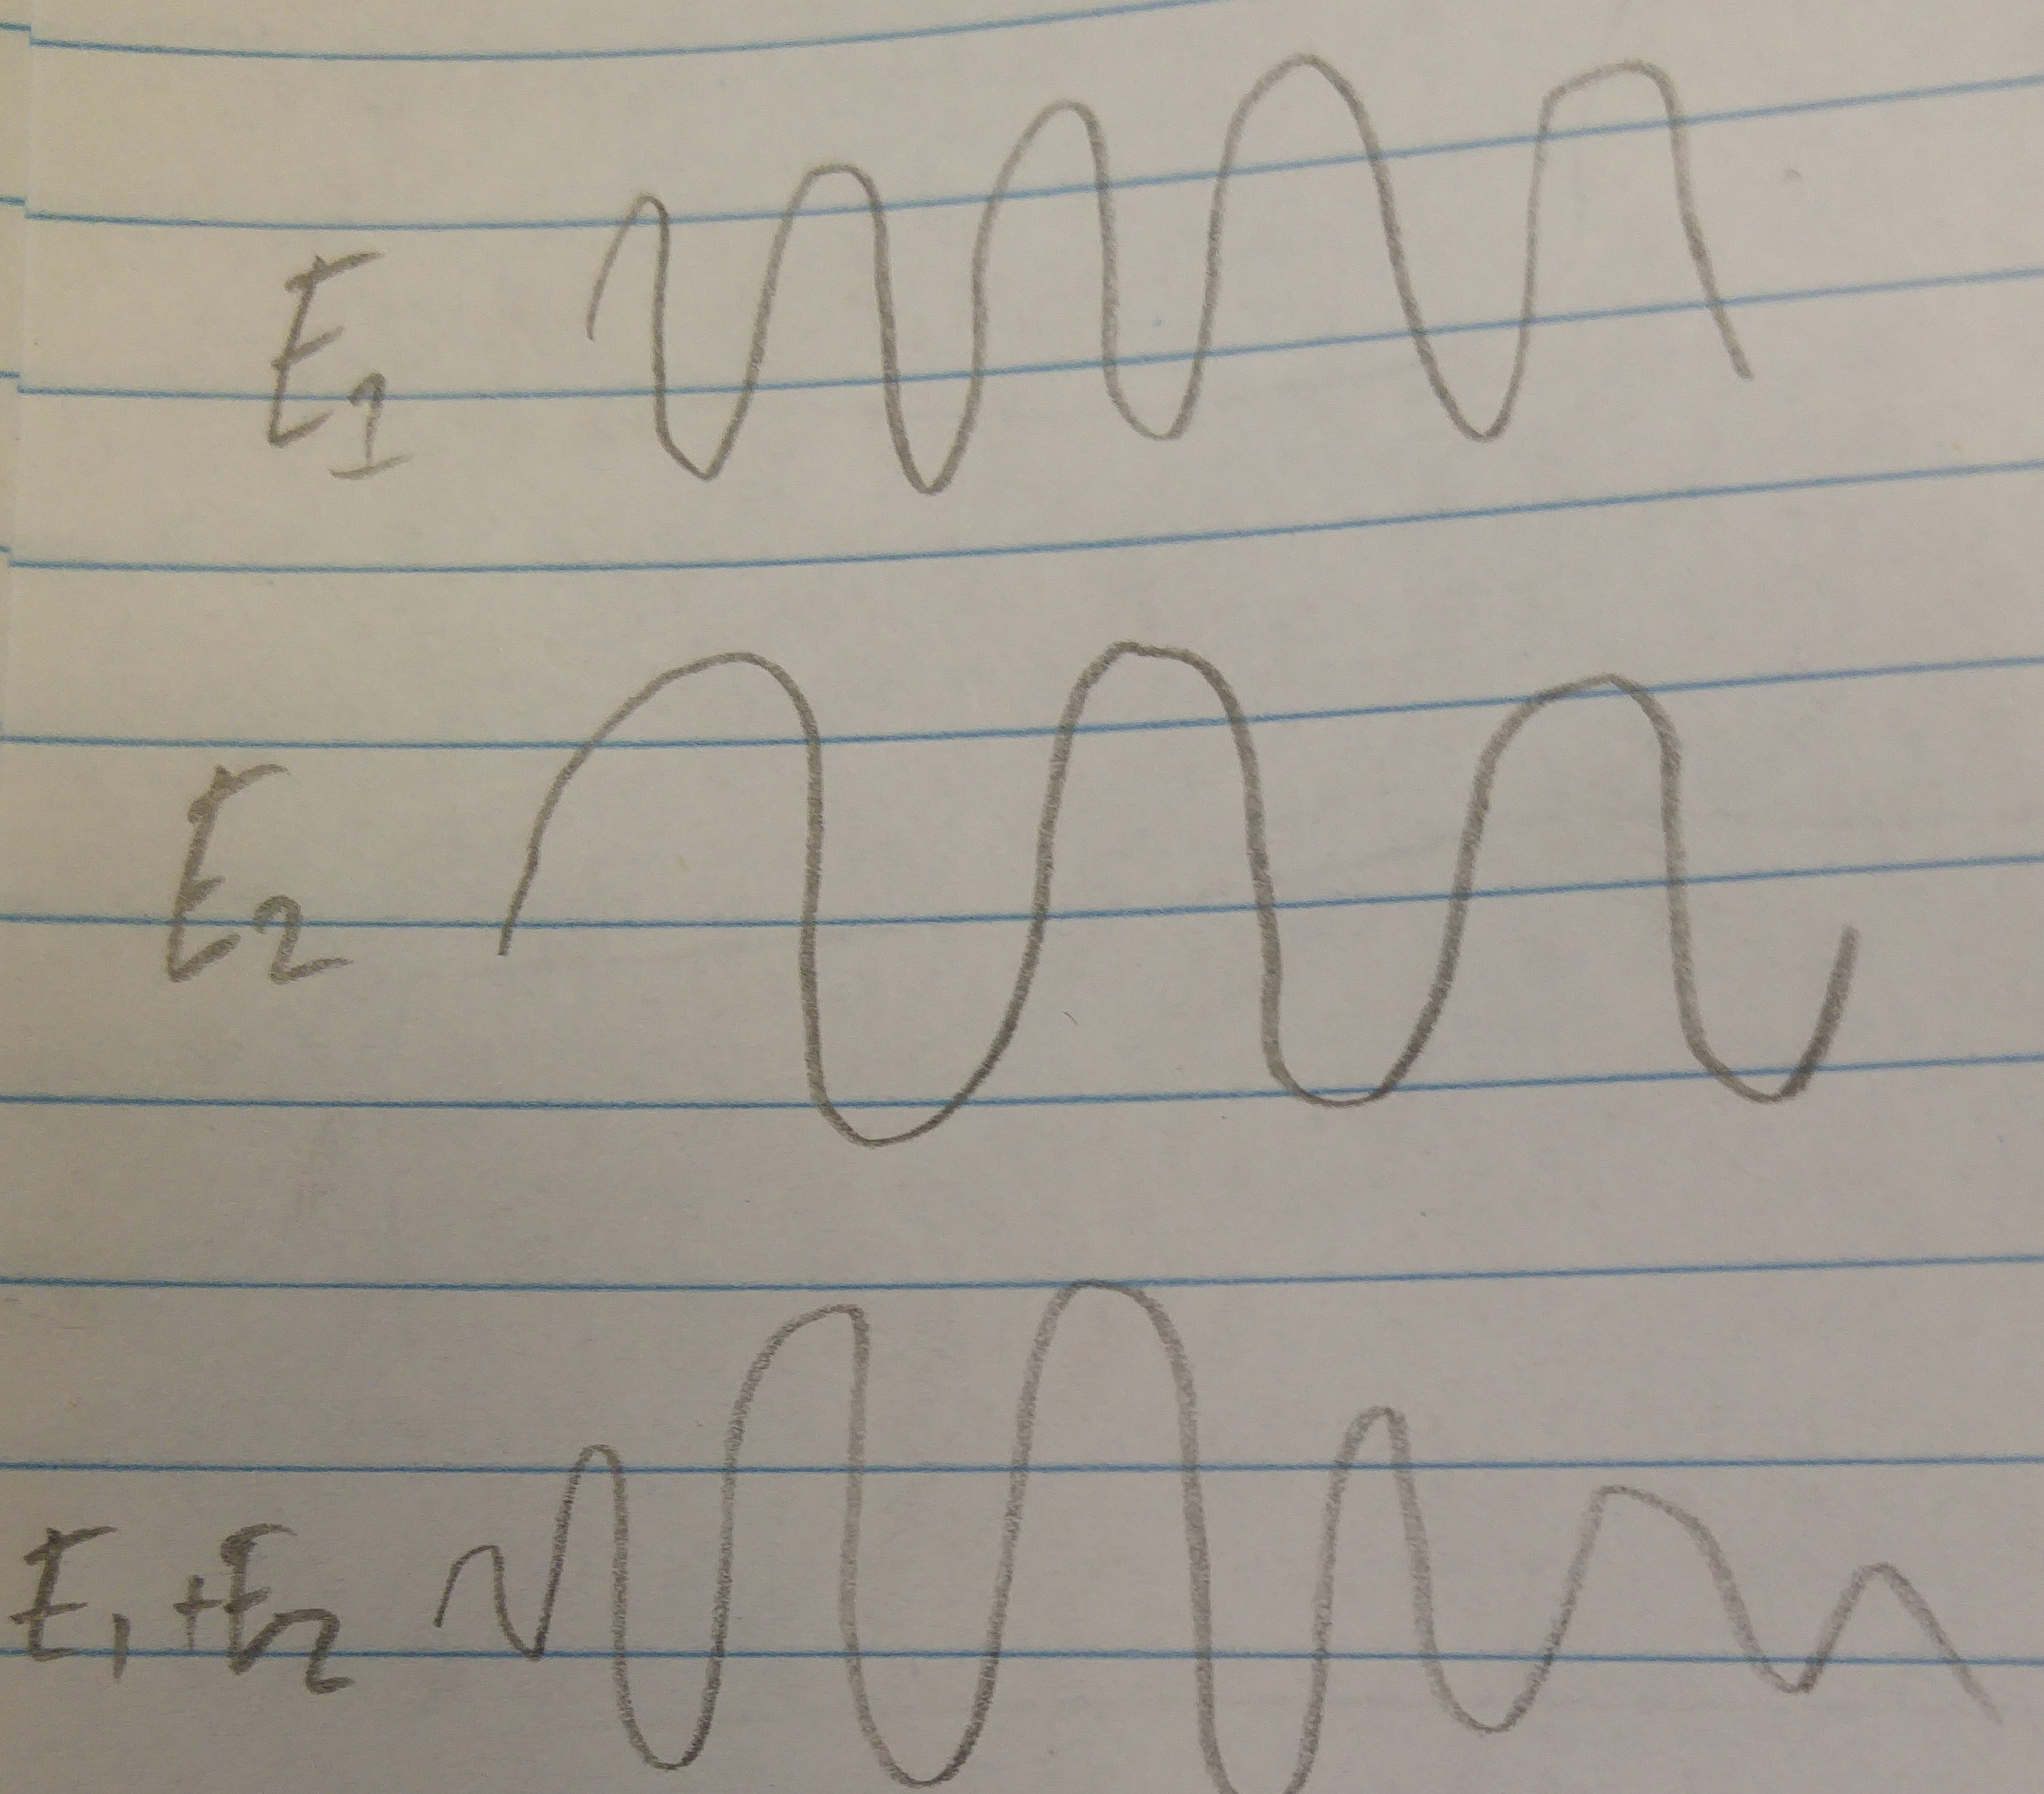
\includegraphics[width=0.5\linewidth]{part1/Figs/beatnote.jpg}
\caption{Depiction of simple beatnote.}
\label{figure:simple_beatnote}
\end{figure}

\subsection{Self-heterodyne}

Self-heterodyne is...

Single delay...

How much delay?

Multipass delay...

These are the results I got...

They look good... too good.

Here's why...\cite{richter_linewidth_1986}

\section{Frequency Reference}
\begin{itemize}
\item Identical laser
\item Narrow laser
\item Three Gaussian lasers
\end{itemize}

\section{Noise measurements}

\section{Bandwidth Stuff}

\section{Long Term Stability}

\subsection{Fibre Stability}

Make some measurements of how the fibres behave over time. Map it to the frequency stability of PS.




\part{Coherent Diffractive Imaging with a Cold-Atom Electron Source}

\appendix
\chapter{Glossary}
\printglossary

% References
%\bibliographystyle{unsrt}
%\renewcommand\bibname{References}
\printbibliography

\end{document}
